\documentclass[]{article}
\usepackage{lmodern}
\usepackage{amssymb,amsmath}
\usepackage{ifxetex,ifluatex}
\usepackage{hyperref}
\usepackage{fixltx2e} % provides \textsubscript
\usepackage{cleveref}
\usepackage{enumitem}
\usepackage{graphicx}
\ifnum 0\ifxetex 1\fi\ifluatex 1\fi=0 % if pdftex
  \usepackage[T1]{fontenc}
  \usepackage[utf8]{inputenc}
\else % if luatex or xelatex
  \ifxetex
    \usepackage{mathspec}
  \else
    \usepackage{fontspec}
  \fi
  \defaultfontfeatures{Ligatures=TeX,Scale=MatchLowercase}
\fi
% use upquote if available, for straight quotes in verbatim environments
\IfFileExists{upquote.sty}{\usepackage{upquote}}{}
% use microtype if available
\IfFileExists{microtype.sty}{%
\usepackage[]{microtype}
\UseMicrotypeSet[protrusion]{basicmath} % disable protrusion for tt fonts
}{}
\PassOptionsToPackage{hyphens}{url} % url is loaded by hyperref
\usepackage[unicode=true]{hyperref}
\hypersetup{
            pdfborder={0 0 0},
            breaklinks=true}
\urlstyle{same}  % don't use monospace font for urls
\IfFileExists{parskip.sty}{%
\usepackage{parskip}
}{% else
\setlength{\parindent}{0pt}
\setlength{\parskip}{6pt plus 2pt minus 1pt}
}
\setlength{\emergencystretch}{3em}  % prevent overfull lines
\providecommand{\tightlist}{%
  \setlength{\itemsep}{0pt}\setlength{\parskip}{0pt}}
\setcounter{secnumdepth}{0}
% Redefines (sub)paragraphs to behave more like sections
\ifx\paragraph\undefined\else
\let\oldparagraph\paragraph
\renewcommand{\paragraph}[1]{\oldparagraph{#1}\mbox{}}
\fi
\ifx\subparagraph\undefined\else
\let\oldsubparagraph\subparagraph
\renewcommand{\subparagraph}[1]{\oldsubparagraph{#1}\mbox{}}
\fi

% set default figure placement to htbp
\makeatletter
\def\fps@figure{htbp}
\makeatother

\title{CS 182: Problem Set 3}
\author{Alan Turing}
\date{\today}

\begin{document}

\maketitle

\textbf{Introduction:}  
Welcome to the third official homework for CS182!  As you are hopefully already aware, this PDF comprises the written component of the second problem set.  In addition to solving the problems found below, you will also need to complete the coding part of the assignment, found in the Github repo.  Finally, we'd like to remind you that while you are allowed a partner for the coding part of the assignment, you are \textbf{NOT} allowed a partner for this and all future written components.  All written work should be yours and yours alone.  This being said, in addition to being able to ask questions at office hours, you are allowed to discuss questions with fellow classmates, provided 1) you note the people with whom you collaborated, and 2) you \textbf{DO NOT} copy any answers.  Please write up the solutions to all problems independently.

\bigskip
\textbf{Collaborators:}

\clearpage

\textbf{Problem 1 (Markov Decision Processes) -- 5 Points:}
Annie is a 5-year old girl who loves eating candy and is ambivalent regarding vegetables. She can either choose to eat candy (Hershey's, Skittles, Peanut Butter Cups) or eat vegetables during every meal. Eating candy gives her +10 in happiness points, while eating vegetables only gives her +4 happiness points. But if she eats too much candy while sick, her teeth will all fall out (she won't be able to eat any more). Annie will be in one of three states: healthy, sick, and toothless. Eating candy tends to make Annie sick, while eating vegetables tends to keep Annie healthy. If she eats too much candy, she'll be toothless and won't eat anything else. The transitions are shown in the table below.

\begin{table}[htb]
\centering
    \begin{tabular}{|c|c|c|c|}
      \hline
        Health condition &	Candy or Vegetables? &	Next condition & Probability \\\hline
        healthy &	vegetables &	healthy & 	1 \\\hline
        healthy &	candy &	healthy & 	1/4 \\\hline
        healthy &	candy &	sick & 	3/4 \\\hline
        sick &	vegetables &	healthy & 	1/4 \\\hline
        sick &	vegetables &	sick & 	3/4 \\\hline
        sick &	candy &	sick & 	7/8 \\\hline
        sick &	candy &	toothless & 	1/8 \\\hline
    \end{tabular}
\end{table}
  
\begin{enumerate}[label=(\alph*)]
    \item (1 Point) Model this problem as a Markov Decision Process: formally specify each state, action, and transition $T(s,a,s')$ and reward $R(a)$ functions.
    \item (1 Point) Write down the Value function $V(s)$ for this problem in all possible states under the following policies: $\pi_1$ in which Annie always eats candy and $\pi_2$ in which Annie always eats vegetables. The discount factor can be expressed as $\gamma$.
    \item (1 Point) Start with a policy in which Annie always eats candy no matter what the her health condition is. Simulate the first two iterations of the policy iteration algorithm. Show how the policy evolves as you run the algorithm. What is the policy after the third iteration? Set $\gamma = 0.9$.
    \item (2 Points) Which of the following five statements are true for an MDP? Select all that apply and briefly explain why.
    \begin{enumerate}[label=(\roman*)]
        \item If one is using value iteration and the values have converged, the policy must have converged as well.
        \item Expectimax will generally run in the same amount of time as value iteration on a given MDP.
        \item For an infinite horizon MDP with a finite number of states and actions and with a discount factor that satisfies 0 < $\gamma$ <= 1, policy iteration is guaranteed to converge.
        \item There may be more than one optimal value function.
        \item There may be more than one optimal policy.
    \end{enumerate}
\end{enumerate}

\bigskip

\textbf{Solution 1:}
% TODO: Your solution to Problem 1

\clearpage

\textbf{Problem 2 (Reinforcement Learning) -- 7 Points:}

\begin{enumerate}[label=(\alph*)]
    \item (1 Point) In class we learned a couple of temporal-difference techniques for reinforcement learning. Now we'd like to take the next step (literally). Suppose we take two steps and get the state/action sequence s-a-s'-a'-s''. Write temporal-difference update equations in terms of $V$.
    \item Consider the following deterministic Transition/Reward Model for an MDP with states (S1, S2, S3, S4, S5, S6) and actions (A1, A2, A3):
    \begin{table}[htb]
    \centering
        \begin{tabular}{|c|c|c|c|}
          \hline
            From &	Action &	To &	Reward \\\hline
            S1 &	A3 &	S2 &	3 \\\hline
            S2 &	A1 &	S1 &	2 \\\hline
            S2 &	A2 &	S3 &	1 \\\hline
            S3 &	A1 &	S4 &	2 \\\hline
            S3 &	A2 &	S5 &	10 \\\hline
            S4 &	A3 &	S3 &	5 \\\hline
            S5 &	A1 & 	S6 &	7 \\\hline
            S6 &	A3 &	S5 &	2 \\\hline
        \end{tabular}
    \end{table}
    \begin{enumerate}[label=(\roman*)]
        \item (1 Point) Suppose we start in state S3. We run Q-learning on this MDP using a greedy policy (always choose action with best Q-value). Ties are given to the action with the lower number (A1 > A2, etc). Assume $\alpha=0.5$ and $\gamma=0.9$. What are the first 4 (state, action) pairs visited, including the start state and the following action?
        \item (1 Point) Why is this simple-greedy policy limited and what can we alter about this algorithm to overcome this limitation? 
    \end{enumerate}
    \item Consider the following Transition/Reward Model for an MDP with states (S1, S2, S3, S4, S5) and actions (A1, A2) -- (S4, S5) are terminal states with no valid actions. Assume $\gamma=1.0$:
    \begin{table}[htb]
    \centering
        \begin{tabular}{|c|c|c|c|c|}
          \hline
            From &	Action &	To &	Reward &	Probability \\\hline
            S1 &	A1 &	S2 &	0 &	0.5 \\\hline
            S1 &	A1 &	S3 &	0 &	0.5 \\\hline
            S1 &	A2 &	S2 &	0 &	0.25 \\\hline
            S1 &	A2 &	S3 &	0 &	0.75 \\\hline
            S2 &	A1 &	S4 &	6 &	1.0 \\\hline
            S2 &	A2 &	S4 &	12 &	0.5 \\\hline
            S2 &	A2 &	S5 &	4 &	0.5 \\\hline
            S3 &	A1 &	S5 &	16 &	1.0 \\\hline
        \end{tabular}
    \end{table}
    \begin{enumerate}[label=(\roman*)]
        \item (1 Point) Compute $Q^*(s,a)$ for each state-action pair using Q-value iteration and show the process.
        \item (1 Point) Compute the optimal policy.
        \item (1 Point) Initialize Q to 0 for all (state, action) pairs for q-learning. With $\alpha = 0.5$, compute Q after seeing:
        [(S1,A1,S2) -> (S2,A2,S4)] 
        [(S1,A2,S3) -> (S3,A1,S5)]
        [(S1,A2,S2) -> (S2,A1,S4)]
        \item (1 Point) Notice that whatever our first action is, the rewards are 0. When we're q-learning regardless of what first action we take, we won't gain much information. Suppose we have an MDP where states can be ordered $S1, S2, S3, ...$ such that there exists no transition $S_i \rightarrow S_j$ for $i > j$. Let's redefine our rewards model to be 
        $$\hat{R}(s,a,s') = Q^*(s,a) - \gamma V^*(s')$$
        so that now our first action is taking into account future rewards. Prove that $\hat{Q}^*(s,a)$ is unchanged, i.e. $\hat{Q}^*(s,a) = Q^*(s,a)$.
    \end{enumerate}
\end{enumerate}

\bigskip

\textbf{Solution 2:}
% TODO: Your solution to Problem 2

\clearpage

\textbf{Problem 3 (Beam Search) -- 2 Points:}
Ant colony optimization is an optimization technique that was inspired by the foraging behavior of real ant colonies. When searching for food, ants initially explore the area surrounding their nest in a random manner. Ants communicate indirectly by means of chemical pheromone trails, which help them find the shortest paths between their nest and the nearest food. While moving, they leave a trail of chemical pheromone behind them. Once an ant finds food, they vary the amount of pheromone they leave depending on the quality and quantity of food. This indirect communication between ants via pheromone trails enables them to find the shortest paths between their nest and the food sources.

\begin{center}
    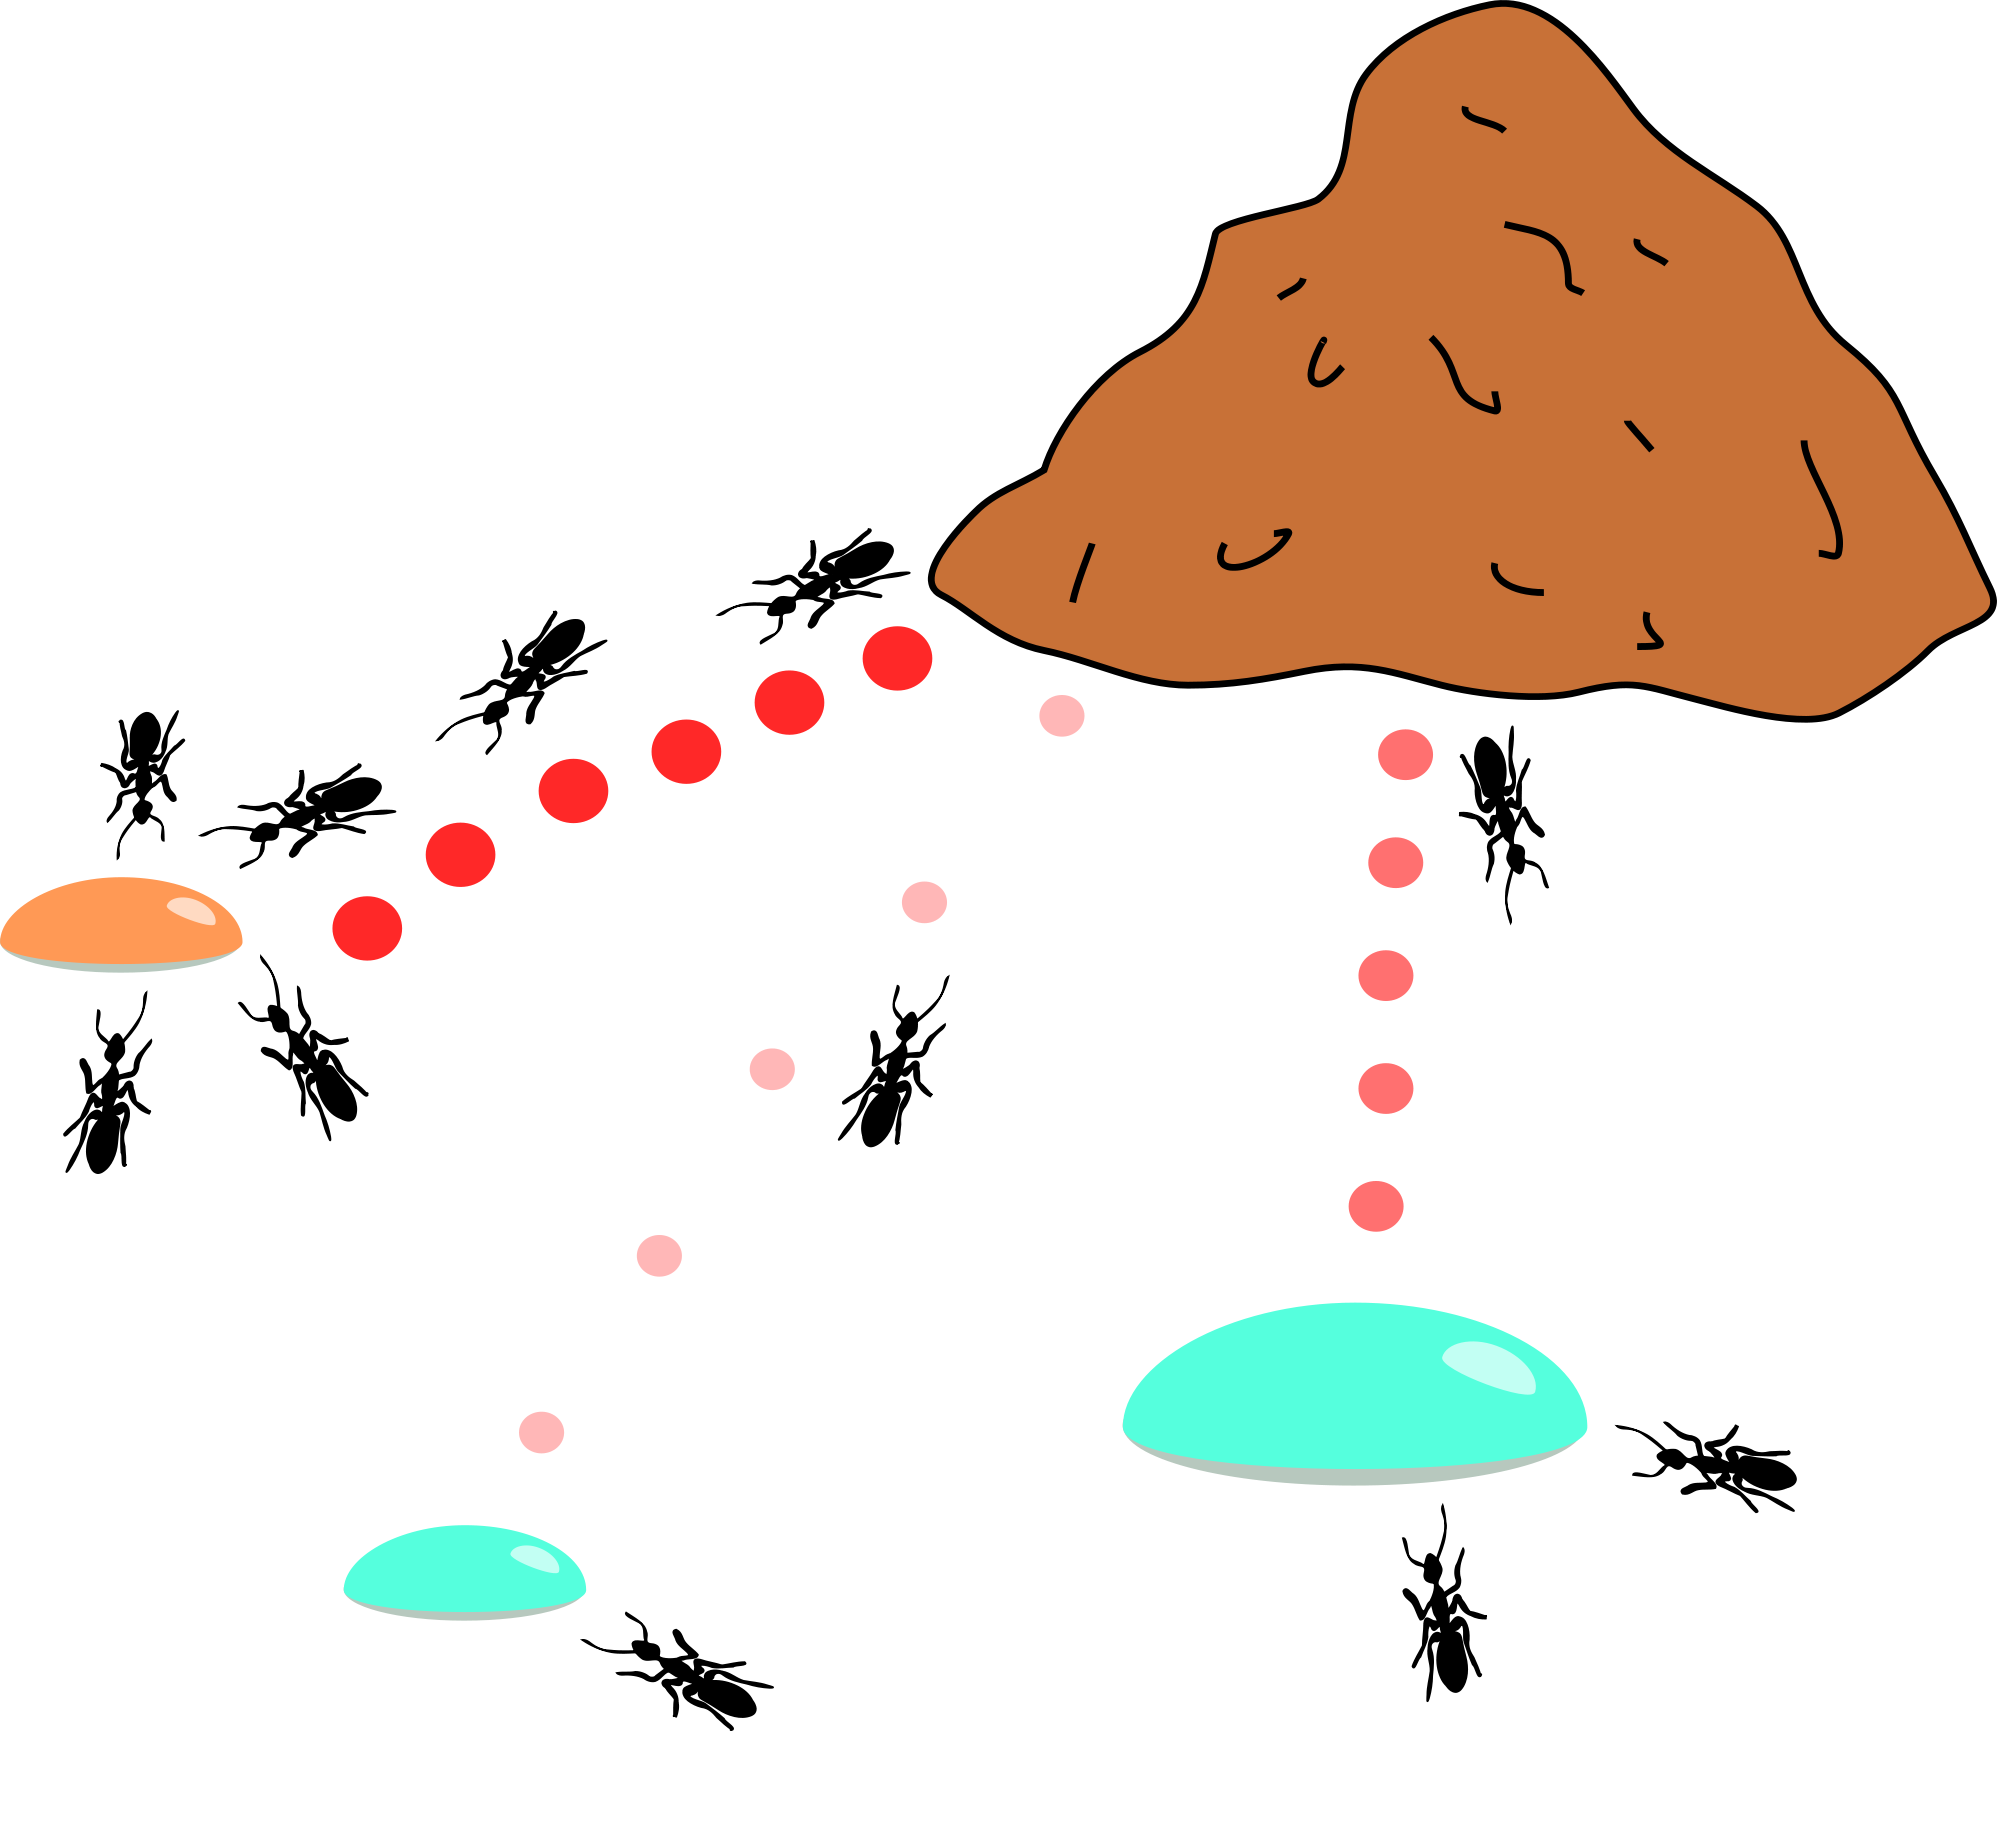
\includegraphics[width=7cm]{ant_colony.png}
\end{center}

Describe (in words) how the ant colony optimization problem can be modeled through a local beam search algorithm. Indicate what $k$ stands for and how the ants find the $k$-best successors for each iteration.

\bigskip

\textbf{Solution 3:}
% TODO: Your solution to Problem 3


\end{document}

